\usepackage[authoryear,round]{natbib}
\usepackage{multirow}

\newcommand{\sheetnum}{%
	06
}
%\setcounter{section}{\sheetnum-3}
\newcommand{\tutorialtitle}{%
    PCA for ICA and Fast ICA
}
\newcommand{\tutorialtitleshort}{%
	PCA for ICA and FastICA
}
% for slides
\subtitle{\sheetnum \tutorialtitle}

%\maxdeadcycles=1000 % Workaround for ! Output loop---100 consecutive dead cycles because of too many figures

% The following use of algroithms does not work well with the notes:
%
%
%
%
% instead use the following for your algorithms:
%
%\begin{figure}[!t]
%\removelatexerror
%\begin{algorithm}[H]
    % your algo here
    %\label{alg:algolabel}
    %\caption{algocaption}
%\end{algorithm}
%\end{figure}
%\begin{algorithm}
% Below is the definition for the command \removelatexerror:
\makeatletter
\newcommand{\removelatexerror}{\let\@latex@error\@gobble}
\makeatother

\begin{document} %%%%%%%%%%%%%%%%%%%%%%%%%%%%%%%%%%%%%%%%%%%%%%%%%%%%%%%

\sheet{\sheetnum}{\tutorialtitleshort}

\ttopic{\tutorialtitle}

\columnratio{0.2,0.8}\textbf{}
\begin{paracol}{2}
%\setlength{\columnseprule}{0.1pt}
%\setlength{\columnsep}{5em}

\begin{rightcolumn}

% notes version will ignore it
\begin{frame}
\titlepage
\end{frame}

\begin{frame}
\tableofcontents
\end{frame}

\newpage

\mode<all>

\section{The ICA Problem}
\begin{frame}

independent sources: $\vec s = (s_1, s_2,...,s_N)^\top \in \R^N$\\
observations: $\vec x \in \R^N$

\begin{equation}
\label{eq:ica}
\vec x = \vec A \, \vec s
\end{equation}

\begin{equation}
\widehat{\vec s} = \vec W \cdot \vec x
\end{equation}

Methods for solving the ICA problem:

\begin{itemize}
\item maximizing the \emph{mutual information} between $\vec x$ and $\vec {\hat s}$ \\
(e.g. Infomax)
\item maximizing the \emph{nongaussianity} of $\widehat {\vec s}$ \\
(e.g. Kurtosis-based ICA, FastICA)
\end{itemize}
\end{frame}

\begin{frame}
\underline{Outline:}
\begin{itemize}
    \item ICA on whitened data
    \begin{itemize}
        \item Whitening/sphering
        \item Amibguities in ICA
        \item PCA is \emph{half} the ICA Problem
    \end{itemize}
    \item the problem with gaussians
    \item maximizing nongaussianity
    \begin{itemize}
        \item Kurtosis-based
        \item negentropy
    \end{itemize}
\end{itemize}
\end{frame}

\newpage
\section{Whitening}

\begin{frame}

\notesonly{
The purpose of whitening is to decorrelate the data.
}

Let the data $\vec X \in \R^{N \times p}$ be centered:

\begin{equation}
\label{eq:centered}
\E \lbrack \vec x \rbrack = 0 
\end{equation}

\notesonly{
From this follows:
}

\begin{equation}
\label{eq:cov}
\vec \Sigma_x = \mathrm{Cov}(\vec x) = \E \lbrack \, \vec x \, \vec x^\top \rbrack 
\end{equation}

The whitening transformation yields:

\begin{equation}
\label{eq:whitening}
\vec v^{(\alpha)} = \vec \Lambda^{-\frac{1}{2}} \vec M^\top \vec x^{(\alpha)}
\end{equation}

where $\vec M = (\vec e_1, \vec e_2, \ldots,\vec e_N)$
\notesonly{
and $\vec \Lambda^{-\frac{1}{2}}$ is a diagonal matrix containig the square roots of the corresponding eigenvalues.
}
\begin{equation}
\label{eq:covw}
\vec \Sigma_v = \mathrm{Cov}(\vec v) = \E \lbrack \, \vec v \, \vec v^\top \rbrack = \vec I_N
\end{equation}

\notesonly{
Uncorrelted means zero covariance. Therefore, the covariance matrix for uncorrelated data is a diagonal matrix because it only contains the variances of the individual variables. 
Whitening decorrelates the variables and normalizes the variances to 1.
}
\end{frame}

\begin{frame}
\begin{figure}[ht]
\label{fig:sphering}
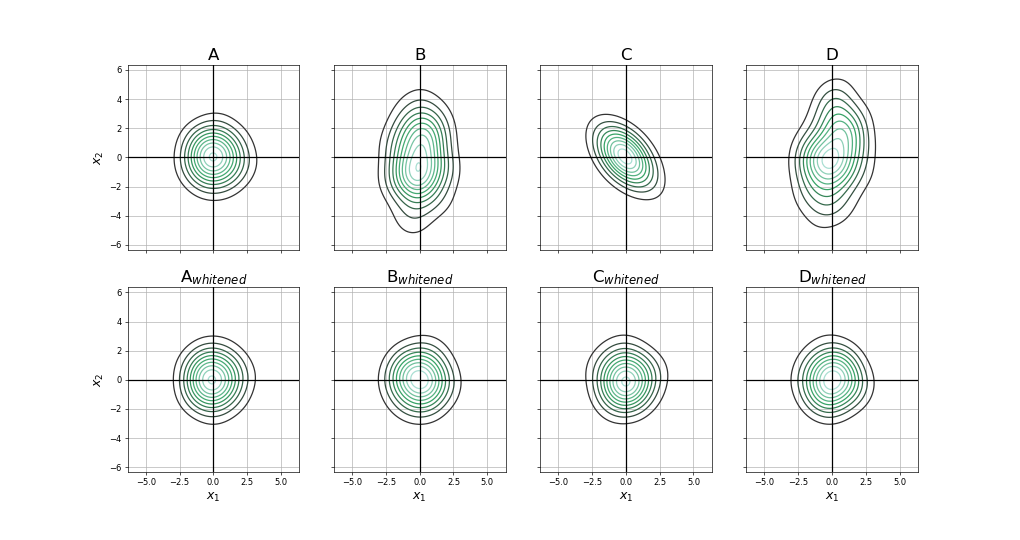
\includegraphics[width=12cm]{img/cov.png}
\caption{A visual interpretation of whitening}
\end{figure}

\end{frame}
\newpage
\section{Ambiguities in ICA and limitations}
\begin{frame}

Sources can be recovered up to:
\begin{itemize}
\item sign
\item scale
\item permutation i.e. ordering
\item only one gaussian distributed source
\end{itemize}
\begin{align*}
\vec P &:= \text{arbitrary permutation matrix}\\
\vec \Lambda &:= \text{arbitrary diagonal matrix}
\end{align*}
\begin{align}
\vec x &= \vec A \, \vec s\\
\vec x &= \lbrack \, \vec A\, \vec P^{-1} \vec \Lambda^{-1}\, \rbrack \, \lbrack \, \vec \Lambda \, \vec P \, \vec s\, \rbrack
\end{align}

\end{frame}



ICA cannot resolve if the mixing matrix is $\vec A$ or a permuatated and/or scaled version of $\vec A$.
It can \textbf{also} not resolve if the independent sources are $\vec s$ or a permutated and/or scaled version of $\vec s$.

Permutations and scaling are not an issue for ICA because permutation and scaling do not interfere with statistical independence.

$$
P_{s_1, s_2}(\widehat {\vec s}) \eqexcl  P_{s_1} (\widehat{s}_1) \cdot P_{s_2} (\widehat{s}_2)
$$

\begin{frame}
Permutations of sources
{\footnotesize
\begin{equation*}
	\arraycolsep=1.4pt%\def\arraystretch{2.2}
	\begin{array}{ccc}
	\left( \begin{array}{ll}
		\textcolor{gray}{\widehat{s}_1} \\ \widehat{s}_2
	\end{array} \right)
	=
	\left( \begin{array}{ll}
	\textcolor{gray}{\mathrm{w}_{11}} & \textcolor{gray}{\mathrm{w}_{12}} \\
		\mathrm{w}_{21} & \mathrm{w}_{22} 
	\end{array} \right)
	\left( \begin{array}{ll}
		\mathrm{x}_1 \\ \mathrm{x}_2
	\end{array} \right)
	& \corresponds &
	\left( \begin{array}{ll}
		\widehat{s}_2 \\ \textcolor{gray}{\widehat{s}_1}
	\end{array} \right)
	 = 
	\left( \begin{array}{ll}
		\mathrm{w}_{21} & \mathrm{w}_{22} \\
		\textcolor{gray}{\mathrm{w}_{11}} & \textcolor{gray}{\mathrm{w}_{12}} 
	\end{array} \right)
	\left( \begin{array}{ll}
		\mathrm{x}_1 \\ \mathrm{x}_2
	\end{array} \right)
	\\\\
	P_{s_1} (\widehat{s}_1) \cdot P_{s_2} (\widehat{s}_2)
	&& 
	P_{s_2} (\widehat{s}_2) \cdot P_{s_1} (\widehat{s}_1)
	\end{array}
\end{equation*}
}
%%%%%%%%%%%%%%%%%%%%%%%%%%%%%%%%%%%%%%%%%%%%%%%%%%%%%%%%%%%%%%%%%%%
Scaling of source amplitudes:

{\footnotesize
\begin{equation*}
	\begin{array}{ccc}
	\arraycolsep=1.4pt
	\left( \begin{array}{ll}
		\widehat{s}_1 \\ \widehat{s}_2
	\end{array} \right)
	=
	\left( \begin{array}{ll}
		\mathrm{w}_{11} & \mathrm{w}_{12} \\
		\mathrm{w}_{21} & \mathrm{w}_{22} 
	\end{array} \right)
	\left( \begin{array}{ll}
		\mathrm{x}_1 \\ \mathrm{x}_2
	\end{array} \right)
	& \corresponds &
	\left( \begin{array}{ll}
		\textcolor{gray}{a}\,\widehat{s}_1 \\ 
                 \textcolor{gray}{b}\,\widehat{s}_2
	\end{array} \right)
	=
	\left( \begin{array}{ll}
		\textcolor{gray}{a}\,\mathrm{w}_{11} & \textcolor{gray}{a}\,\mathrm{w}_{12} \\
		\textcolor{gray}{b}\,\mathrm{w}_{21} & \textcolor{gray}{b}\,\mathrm{w}_{22} 
	\end{array} \right)
	\left( \begin{array}{ll}
		\mathrm{x}_1 \\ \mathrm{x}_2
	\end{array} \right)
	\\\\
	P_{s_1} (\widehat{s}_1) \cdot P_{s_2} (\widehat{s}_2)
	&& 
	aP_{s_1} (a\widehat{s}_1) \cdot bP_{s_2} (b\, \widehat{s}_2)
	\end{array}
\end{equation*}
}
\end{frame}
\subsection{Implications of the ambiguities}

\begin{frame}

We can assume:
$$
\E \lbrack \, \vec s \, \rbrack = 0
$$

Removing the mean from $\vec x$ does not change $\vec A$:

$$
\vec x - \E \lbrack \, \vec x \, \rbrack = \vec A \left( \vec s - \E \lbrack \, \vec s \, \rbrack \right)
$$

\notesonly{Note that} $\E \lbrack \, \vec s \, \rbrack$ and $\E \lbrack \, \vec x \, \rbrack$ are not necessarily equal.
\pause

We can also assume:
$$
\mathrm{Cov}(\vec s) = \E \lbrack \, \vec s \, \vec s^\top \rbrack = \vec I_N
$$

Any scaling in $\mathrm{Cov}(\widehat{\vec s})$ can be assumed to come from $\vec A$ and can be undone.

\end{frame}


\subsection{Whitening in the context of ICA}

\begin{frame}

\begin{align}
\label{eq:expxina}
\vec \Sigma_x = \mathrm{Cov}(\vec x) &=  \E \lbrack \, \vec x \, \vec x^\top \rbrack\\
&=  \E \lbrack \, \vec A\,\vec s \, \left( \vec A\,\vec s \right)^\top \rbrack\\
&=  \E \lbrack \, \vec A\; \underbrace{\;\vec s \, \vec s^\top}_{= \vec I_N} \vec A^\top \rbrack\\
\label{eq:sigmax}
&=  \vec A\, \vec A^\top
\end{align}

\end{frame}

\begin{frame}

\notesonly{
If we were to apply \emph{Singular Value Decomposition} on the symmetric matrix $\Sigma_x$:
}

\begin{equation}
\mathrm{SVD}(\vec \Sigma_x) = \vec U\, \vec D \, \vec U^\top
\end{equation}

where\\
\notesonly{
$\vec U$ is an orthogonal matrix,} $\vec U^\top\vec U = \vec I_N$ and
\notesonly{$\vec D$ is a diagonal matrix with rank $N$, }$\vec D^\top = \vec D$.\\

We define the two following transformation $\vec Q$ and $\widetilde{\vec A}$:
\begin{equation}
\label{eq:defq}
\vec Q := \vec D^{-\frac{1}{2}} \vec U^\top
\end{equation}
\begin{equation}
\label{eq:defatilde}
\widetilde{\vec A} := \vec Q \, \vec A 
\end{equation}

Which yields a new ICA problem:
\begin{equation}
\vec u = \vec Q\, \vec x = \vec Q\,\vec A \, \vec s = \widetilde{\vec A} \, \vec s
\end{equation}

\question{What is so special about the new mixing matrix $\widetilde{\vec A}$?} \\

\notesonly{-$\widetilde{\vec A}$ is orthogonal (i.e. $\widetilde{\vec A}\, \widetilde{\vec A}^\top = \widetilde{\vec A}^\top \widetilde{\vec A} = \widetilde{\vec A}^{-1} \widetilde{\vec A} = \vec I_N$).
 We will see the implications of this in how it reduces the number of free parameters for solving the new ICA problem.
 }
\end{frame}

\begin{frame}

\slidesonly{
$$
\vec Q := \vec D^{-\frac{1}{2}} \vec U^\top
$$
$$
\vec \Sigma_x = \E \lbrack\, \vec x \, \vec x^\top \rbrack = \vec U \, \vec D \, \vec U^{\top}
$$
}

\begin{align}
\E \lbrack\, \vec u \, \vec u^\top \rbrack
&\mystackrel{\vec u = \vec Q\, \vec x}{\vec u = \vec Q\, \vec x}
 \E \lbrack\, \vec Q \, \vec x  \left( \vec Q \, \vec x\right)^\top \rbrack\\
&\mystackrel{\vec u = \vec Q\, \vec x}{}\E \lbrack\, \vec Q \, \vec x \; \vec x^\top \vec Q^\top \rbrack\\
&\mystackrel{\vec u = \vec Q\, \vec x}{} \E \lbrack\, \vec Q \, \vec \Sigma_{X} \, \vec Q^\top \rbrack\\
&\mystackrel{\vec u = \vec Q\, \vec x}{} \vec Q \, \vec \Sigma_{x} \, \vec Q^\top\\
&\mystackrel{\vec u = \vec Q\, \vec x}{}
\left( \vec D^{-\frac{1}{2}} \vec U^\top \right)
\left( \vec U \, \vec D \, \vec U^\top \right)
\left( \vec D^{-\frac{1}{2}} \vec U^\top \right)
\end{align}

\end{frame}
\begin{frame}

\slidesonly{
\begin{align}
\E \lbrack\, \vec u \, \vec u^\top \rbrack
&\mystackrel{\vec u = \vec Q\, \vec x}{}
\left( \vec D^{-\frac{1}{2}} \vec U^\top \right)
\left( \vec U \, \vec D \, \vec U^\top \right)
\left( \vec D^{-\frac{1}{2}} \vec U^\top \right)
\end{align}
}

From $\vec U^\top\vec U = \vec I_N$ and $\vec D^\top = \vec D$ follows:

\begin{align}
\E \lbrack\, \vec u \, \vec u^\top \rbrack
&=
\vec D^{-\frac{1}{2}}
\underbrace{\left( \vec U^\top  \vec U \right)}_{= \vec I_N}
\, \vec D \, 
\underbrace{\left( \vec U^\top \,  \vec U \right)}_{= \vec I_N}
\,
\left(\vec D^{-\frac{1}{2}} \right)^\top \\
&= \vec D^\top
\, 
\underbrace{\vec D^{-\frac{1}{2}}  \, 
\left(\vec D^{-\frac{1}{2}} \right)^\top}_{=\vec D^{-1}} = \vec I_N
\end{align}


Recall 
\notesonly{from \eqref{eq:sigmax}:}
$$
\vec \Sigma_x =  \E \lbrack \, \vec x \, \vec x^\top \rbrack
=  \vec A\, \vec A^\top
$$
Therefore:
$$
\E \lbrack \, \vec u \, \vec u^\top \rbrack
= \widetilde {\vec A}\, \widetilde {\vec A}^\top = \vec I_N
$$

\notesonly{
The new mixing matrix}
$\widetilde{\vec A}$ is orthonormal.\\
The space of solutions is restricted to $\vec W$ that are orthogonal. 
The can speed up convergence of ICA. 
The number of free parameters 
\notesonly{
for solving the new ICA problem 
$\vec u = \widetilde{\vec A}\, \vec s$ 
is reduced from $N^2$ to $N(N-1)/2$
}
\slidesonly{
$N^2 \rightarrow N(N-1)/2$
}
\end{frame}

\begin{frame}
\slidesonly{
\frametitle{What just happend?}

\begin{itemize}
\setlength\itemsep{1em}
\item We've transformed $\vec x$ to get $\vec u$:
$ \qquad \qquad \qquad
\vec u := \vec D^{-\frac{1}{2}} \vec U^\top \vec x
$

\item Where did $\vec D$ and $\vec U$ come from?
$ \qquad \qquad
\mathrm{SVD}(\vec \Sigma_x) = \vec U\, \vec D \, \vec U^\top
$

\item What do $\vec D$ and $\vec U$ represent? - the eigenval. and eigenvect. of $\vec \Sigma_x$

\item What's so special about $\vec u$?
$ \qquad \qquad \qquad \qquad
\vec \Sigma_u = \vec I_N
$

\item ...So?

- new ICA problem: $\vec u := \widetilde{\vec A}\, \vec s$\\
- $\widetilde{\vec A}$ is orthogonal\\
- unmixing the new problem involves only ``half'' the number of weights.

\question{What is the transformation $\vec D^{-\frac{1}{2}} \vec U^\top$ called?}

\end{itemize}
}

\end{frame}


\section{Summary so far:}

\slidesonly{
\begin{frame}
\begin{enumerate}
\item Initial ICA Problem: $\vec x = \vec A\, \vec s$
\item New ICA Problem: $\vec u := \widetilde{\vec A}\, \vec s$,\\

where $\vec u = \vec D^{-\frac{1}{2}} \vec U^\top \vec x$ and $\vec \Sigma_u = \vec I_N$.
\item $\vec u$ is the \emph{whitened} version of $\vec x$.
\item $\vec D$ and $\vec U$ can be obtained via PCA on $\vec x$.
\item Applying ICA on whitened data reduces the number of free parameters.
\item PCA simplifies the ICA problem.
\item ICA on whitened data is about ``rotating'' it back.
\end{enumerate}

\end{frame}
}
\subsection{Gaussians are bad for ICA}

\begin{frame}

\textbf{A visual argument:}

\notesonly{Consider the following uniformly distributed independent sources $s1$ and $s2$ and corresponding arbitrary mixtures $x_1$ and $x_2$:
}
\slidesonly{
Mixing uniformly distributed independent sources $s1$ and $s2$:
}

\begin{tabular}[h]{c c}
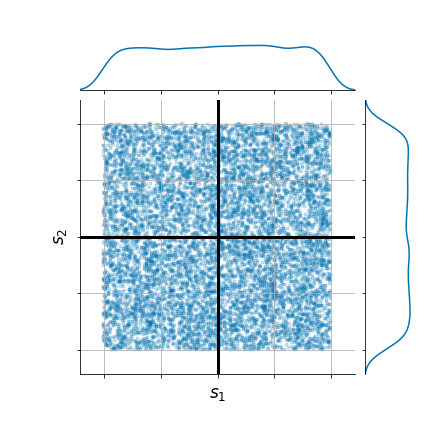
\includegraphics[width=4.5cm]{img/uniform-s_centered.png} &
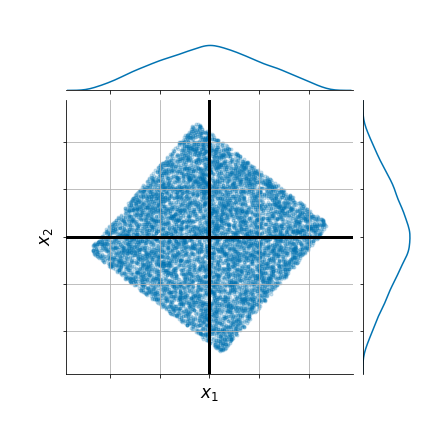
\includegraphics[width=4.5cm]{img/uniform-x_whitened.png}\\
original $\vec s$& $\vec x = \vec A \, \vec s$ 
\end{tabular}

\notesonly{The task of ICA is to find an unmixing matrix $\vec W$ that rotates $\vec x$ back to its original orientation. 
If the density $\vec x$ were to follow more the shape of a rectangle or parallelogram, whitening 
would decorrelate the data and normalized the variances such that the density appears as a square, which then reduces the ICA problem, of finding the right rotation. 
The same applies to other densities (not necesarly shaped as rectangles or squares) in that ICA on whitened data ``rotates things back''.}
\end{frame}

\begin{frame}
\slidesonly{
\frametitle{Gaussians are bad for ICA}
}
\notesonly{
If our independent sources were normally distributed (left), a mixing matrix will effectively rotate in some way, which yields the same circular ``shape'':

}
\slidesonly{
Mixing normally distributed independent sources $s1$ and $s2$:
}
\begin{tabular}[h]{c c}
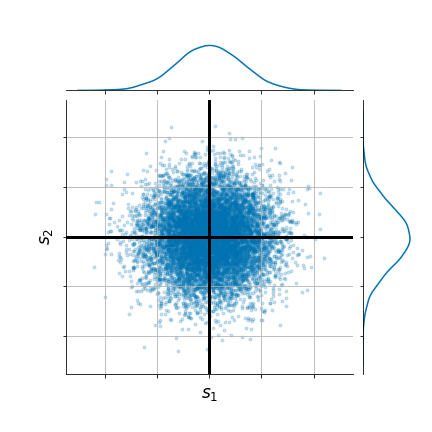
\includegraphics[width=4.5cm]{img/normal-s_centered.png} &
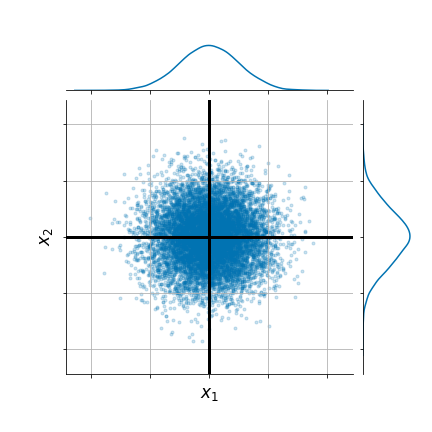
\includegraphics[width=4.5cm]{img/normal-x_whitened.png}\\
original $\vec s$& $\vec x = \vec A \, \vec s$ 
\end{tabular}

\question{How should we rotate $\vec x$ to get back $\vec s$?}
\pause
\notesonly{It's not possible. The gaussian distribution is \emph{rotationally symmetric}. We cannot resolve the original axes.
}
\end{frame}

\begin{frame}
\slidesonly{
\frametitle{Gaussians are bad for ICA}
}
\newpage
\textbf{A more formal argument for why Gaussians are bad for ICA}:

Recall that the joint density of independent sources is a factorizing density:

\begin{equation}
\label{eq:facts}
P_{\vec s}(\vec s) = \prod_{i=1}^{N} P_{s_i}(s_i)  \,.
\end{equation}

If we assumed gaussian distributed sources, the following factorization becomes possible:

\begin{equation}
	\label{eq:factsgauss}
	\begin{array}{ll}
	P_{\vec{s}}({\vec{s}}) 
	& = \frac{1}{2\pi} 
    \exp \left( -\frac{\lVert{\vec{s}}\rVert^2}{2} \right)
	\\
	& = \underbrace{
	\Bigg[ \frac{1}{\sqrt{2\pi}} \exp \left( -
		\frac{{s_1}^2}{2} \right) \Bigg]
		}_{{P}_{s_1}({s}_1)}
		\underbrace{\Bigg[
			\frac{1}{\sqrt{2\pi}} \exp \left( -
			\frac{{s_2}^2}{2} \right)
		\Bigg]
			}_{{P}_{s_2}({s}_2)}
	\end{array}
\end{equation}
\end{frame}

\begin{frame}
\slidesonly{
\frametitle{Gaussians are bad for ICA}
}
\slidesonly{\textbf{A more formal argument (cont'd):}}

Now consider applying an orthognal mixing matrix that is \textbf{known}. 
\slidesonly{(orthogonal from whitening the $\vec x$)\\
Consequently:
}
\notesonly{We've seen how whitening takes an ICA problem with any valid\footnote{invertible} mixing matrix $A$ 
and reformulates it into a new problem with an orthogonal mixing matrix $\widetilde{\vec A}$.
The following holds for such an orthogonal mixing matrix $\widetilde{\vec A}$:
}
$$
\widetilde{\vec A}^\top = \widetilde{\vec A}^{-1} \Leftrightarrow \widetilde{\vec A}^{-1}\widetilde{\vec A}=\vec I_N \qquad \text{and} \qquad |\det \widetilde{\vec A}| = |\det \widetilde{\vec A}^\top| = 1
$$

$$
\vec s = \widetilde{\vec A}^{-1} \vec{x} = \widetilde{\vec A}^\top \vec x
$$

\notesonly{
We are now interested in the joint density $P_x(\vec x)$ of the mixtures $x_1$ and $x_2$.
}

Density transformation tells us that:
\begin{equation}
	\label{eq:gausstransformeddt}
	{P}_{\vec x}(\vec x) = 
    {P}_{\vec s}(\vec s)  \left|\det \frac{\partial \vec s}{\partial \vec x}\right| 
    = {P}_{\vec s}(\vec s)  \left|\det  \widetilde{\vec A}^{-1}\right|
    = {P}_{\vec s}(\vec s)  \left|\det  \widetilde{\vec A}^\top\right|
\end{equation}
Therefore,
\slidesonly{
\begin{equation}
	{P}_{\vec x}(\vec x)
	= \frac{1}{2\pi} 
    \exp \left( 
    -\frac{\lVert{\widetilde{\vec A}^\top \vec x}\rVert^2}{2} 
    \right)
    \left|\det  \widetilde{\vec A}^\top\right|
	= \ldots?
\end{equation}
}
\end{frame}

\begin{frame}
\slidesonly{
Orthogonal mixing matrix $\widetilde{\vec A}$ implies:
$$
\widetilde{\vec A}^\top = \widetilde{\vec A}^{-1} \Leftrightarrow \widetilde{\vec A}^{-1}\widetilde{\vec A}=\vec I_N \qquad \text{and} \qquad |\det \widetilde{\vec A}| = |\det \widetilde{\vec A}^\top| = 1
$$
$$
\vec s = \widetilde{\vec A}^{-1} \vec{x} = \widetilde{\vec A}^\top \vec x
$$}
\begin{align}
    \label{eq:gaussx}
	{P}_{\vec x}(\vec x)
	&= \frac{1}{2\pi} 
    \exp
    \Big(
    -\frac{
    \overbrace{
    \lVert{\widetilde{\vec A}^\top \vec x}\rVert^2
    }^{\mathclap{
		\lVert{\widetilde{\vec A}^\top \vec x}\rVert^2
		= \left(\widetilde{\vec A}^\top \vec x\right)^\top \widetilde{\vec A}^\top \vec x
		\,=\, \vec x^\top \widetilde{\vec A} \, \widetilde{\vec A}^\top \vec x
		= \vec x^\top \vec x
		= \lVert{\vec x}\rVert^2
		}}}{2}
    \Big)
    \underbrace{
    \left|\det  \widetilde{\vec A}^\top\right|
    }_{=\, 1}
    \\
	&= \frac{1}{2\pi} 
    \exp \left( 
    -\frac{\lVert{\vec x}\rVert^2}{2} 
    \right)\\
    \label{eq:gaussxfact}
	& = \underbrace{
	\Bigg[ \frac{1}{\sqrt{2\pi}} \exp \left( -
		\frac{{x_1}^2}{2} \right) \Bigg]
		}_{{P}_{x_1}({x}_1)={P}_{s_1}({s}_1)}
		\underbrace{\Bigg[
			\frac{1}{\sqrt{2\pi}} \exp \left( -
			\frac{{x_2}^2}{2} \right)
		\Bigg]
			}_{{P}_{x_2}({x}_2)={P}_{s_2}({s}_2)}
            \text{no change in pdf!}
\end{align}
\end{frame}

We see that the factorization in \eqref{eq:gaussxfact} describes the pdf for the mixtures $\vec x$ identically to the pdf of the original sources. 
The original and mixed distributions are identical. The mixing matrix did not change this. Therefore, it would be impossible to find its corresponding unmixing matrix to undo the rotation.

\begin{frame}
\slidesonly{
\frametitle{Gaussians are bad for ICA}
}

\notesonly{
Mixing two independent Gaussians leads to a joint mixed distribution that is equal to that of the original sources.
This is actually justified by the property that \emph{
uncorrelated jointly Gaussian variables are necessarily independent.}\footnote{
Further details can be found in Hyv{\"a}rinen Ch. 2.5.
}
}

A mixture of sources where at most one is Gaussian, is still fine. It only becomes a problem when we have more than one.


\slidesonly{
\begin{itemize}
\item Mixing two independent Gaussians leads to a joint mixed distribution that is equal to that of the original sources.
\item No surprise: \emph{uncorrelated jointly Gaussian variables are necessarily independent.}
\item One Gaussian + other distributions is fine.
\item Two ore more Gaussians. No way.
\end{itemize}
}
\end{frame}


\section{Solving ICA by maximizing nongaussianity}

\begin{frame}

\begin{block}{Intuition from the Central Limit Theorem}
\emph{The distribution of the sum of independent random variables is ``more Gaussian'' than the original distributions of the random variables.}\\\vspace{2mm}

Searching for the direction of maximum deviation from a Gaussian distribution may recover the original sources.
\end{block}
\end{frame}


\begin{frame}
\frametitle{Maximizing nongaussianity leads to independent sources}

\textbf{The setting:}\\

Two statistically independent sources with $\langle s_i s_j \rangle = \delta_{ij} \quad \Leftrightarrow \quad \langle \vec s \, \vec s^\top \rangle = \vec I_N$
\notesonly{
The sources are mixed using a mixing matrix $\vec A$ resulting in observations $\vec x$:
}
\begin{equation}
\label{eq:icaproblemx}
\vec x = \vec A \, \vec s
\end{equation}
\notesonly{
One out of the $N$ independent sources can be reconstructed using a row vector from an unmixing matrix $\vec W$:
}
\begin{equation}
\label{eq:singlesource}
\widehat s_i = \vec w_i^\top \vec x
\end{equation}
\notesonly{
By substituting \eqref{eq:icaproblemx} for $\vec x$ in \eqref{eq:singlesource}, 
we describe each reconstructed source $\widehat s_i$ as a linear combination of the original sources:
}


\notesonly{According to the CLT we can think of the variables in $\vec x$ to be more Gaussian distributed than the original variables in $\vec s$. 
Therefore, a solution to the ICA problem is finding an inverse to $\vec A$ that undoes this effect and removes the ``accumulated Gaussianity'' from $\vec x$. 
The role of any $\vec w_i$ becomes to maximize the nongaussianity of $\widehat{s}_i$ when we multiply it by $\vec x$. This is the same role $w_i^\top \vec A = \vec z_i^\top$ has when applied to $\vec s$.


}


\begin{equation}
\label{eq:szs}
\widehat s_i = \vec w_i^\top \vec A \, \vec s = \vec z_i^{\top} \vec s = 
	\left( \begin{array}{ll}
		{z}_1 \\ {z}_2
	\end{array} \right)^\top_i
	\left( \begin{array}{ll}
		{s}_1 \\ {s}_2
	\end{array} \right)
= z_1 s_1 + z_2 s_2
\end{equation}

\notesonly{
Looking at \eqref{eq:szs} we recognize that $\vec z_i$ describes how to route the information in $\vec s$ such that $\widehat{\vec s}_i$ fully describes 
one of the independent sources in $\vec s$.
This can be accomplished with a vector containing a single non-zero element:
}

\begin{equation*}
	\vec{z}_{\text{opt.}} = \left( \begin{array}{c}
			0 \\ \pm 1 
		\end{array} \right)
	\quad \text{ or }\quad 
	\vec{z}_{\text{opt.}} = \left( \begin{array}{c}
			\pm 1 \\ 0 
		\end{array} \right)
\end{equation*}

\end{frame}

\notesonly{
Recall that ICA cannot resolve scale or permutation of the sources and thirdly it cannot resolve the sign. 
This is not an issue. 
The role of $\vec z_i$ is to route either $s_1$ or $s_2$ to $\widehat{\vec s}_i$. This covers the ambiguitiy in terms of permutation. 
We cannot have both independent sources contribute to $\widehat{s}_i$, only one can. Therefore, we only need a single non-zero component for $\vec z_i$.
Wether $s_1$ is scaled by any factor before reaching $\widehat{s}_i$ does not make it more or less independent of $s_2$. Choosing $1$ for the non-zero component is therefore sufficient.
Finally, negating the source by multiplying it by $(-1)$ also has no consequences on the independence criterion.

We won't actually try and find $\vec z_i$ because we don't have $\vec s$ to apply them to. We use the requirements for $\vec z_i$ by finding a $\vec w_i$ that satisfies these requirements through:
\begin{equation}
\label{eq:zfromw}
\vec z_i = \left(\vec w_i^\top \vec A\right)^\top =  \vec A^\top \vec w_i
\end{equation}
}

\begin{frame}
\question{Does maximizing nongaussianity deliver independent components?}
\slidesonly{

\begin{equation}
\widehat s_i = \vec z_i^{\top} \vec s = z_1 s_1 + z_2 s_2
\end{equation}

\begin{equation*}
	\vec{z}_{\text{opt.}} = \left( \begin{array}{c}
			0 \\ \pm 1 
		\end{array} \right)
	\quad \text{ or }\quad 
	\vec{z}_{\text{opt.}} = \left( \begin{array}{c}
			\pm 1 \\ 0 
		\end{array} \right)
\end{equation*}

$\vec z_i$ ensures independent $\widehat s_i$

\begin{equation}
\widehat s_i = \vec w_i^\top \vec x
\end{equation}

$\vec w_i$ finds less gaussian $\widehat s_i$

\begin{equation}
\vec z_i =  \vec A^\top \vec w_i
\end{equation}

Maximizing nongaussianity is ensured to keep $\widehat s_i$ independent.

}
\end{frame}
\notesonly{
- By (1) maximizing the nongaussianity of $\vec w_i^\top \vec x$ and (2) having $\vec z_i = \vec A^\top \vec w_i$ yield independent components and (3) knowing that 
$\widehat s_i = \vec w_i^\top \vec x = \vec z_i^{\top} \vec s$, we conclude that maximizing $\vec w_i^\top \vec x$ gives us one independent component.
}
\newpage

\section{Kurtosis as a measure for nongaussianity}

\begin{frame}

\notesonly{
Kurtosis represents the fourth-order cumulant\footnote{
Cumulants allow us to express the i-th moment in terms of a cumulative sum of the moments preceeding it. 
This simplifies the expression of higher-order moments such as kurtosis which is the fourth-order moment.
} of a random variable.
}

\begin{block}{Definition}
	Let $x$ be a random variable with zero-mean, i.e. $\E \lbrack\,x\,\rbrack = 0$.
    \begin{equation}
    \label{eq:kurt}
        \kurt (x) = \langle x^4 \rangle - 3 
            \left( \langle x^2 \rangle \right)^2  \quad
                    \stackrel{\text{sphered data}}{=} \quad \langle x^4 \rangle - 3 
    \end{equation}
    
    \notesonly{
    By assuming zero-mean and unit-variance, we see that kurtosis is simply a normalized version of the fourth moment.
    
    Useful properties of kurtosis:
    
    }
    Let $x_1$ and $x_2$ be two independent random variables, then:
    \begin{eqnarray*}
    \kurt(x_1 + x_2)& = & \kurt(x_1) + \kurt(x_2) \\
    \kurt(z_1 x_1)  & = & z_1^4 \kurt(x_1)
    \end{eqnarray*}
\end{block}
\end{frame}

\begin{frame}

\question{What does kurtosis measure?}\\

\begin{tabular}[h]{c c c c}
&
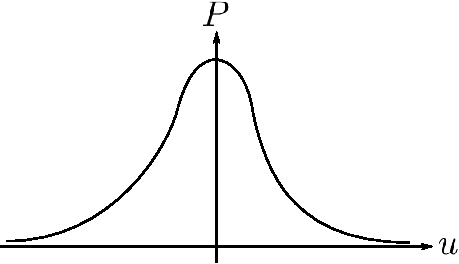
\includegraphics[width=2.7cm]{img/section2_fig20} &
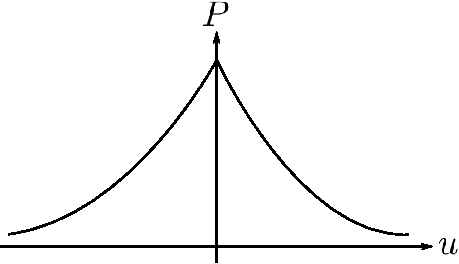
\includegraphics[width=2.7cm]{img/section2_fig21} & 
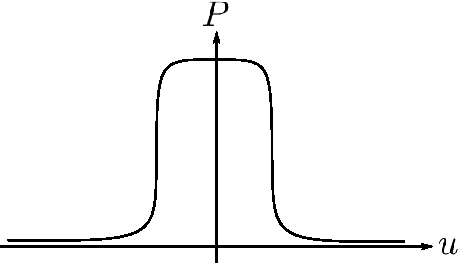
\includegraphics[width=2.7cm]{img/section2_fig22} \\ \\

& $\kurt(x) = 0$ & $\kurt(x) > 0$ & $\kurt(x) < 0$\\ \\

&
Gaussian PDF &
super-Gaussian PDF&
sub-Gaussian PDF\\
&bell shaped & peaky, long tails (``outliers'')& bulky, no ``outliers'' \\\\
e.g.&normal & Laplace & uniform
\end{tabular}\\[1cm]

\notesonly{This implies that we can use}
$|kurt(x)| > 0$ as a measure of nongaussianity 

\textbf{Caveat:}
\slidesonly{
sensitive to outliers
}
\end{frame}


\notesonly{
Kurtosis, just like other higher-order cumulants are sensitive to outliers, in that an outlier
 will register a much higher kurtosis value. This will be addressed later by FastICA.
}

\newpage

\subsection{kurtosis-based ICA}

\begin{frame}

Two statistically independent sources with

$\langle s_i s_j \rangle = \delta_{ij} \quad \Leftrightarrow \quad \langle \vec s \, \vec s^\top \rangle = \vec I_N$ (any scaling can be attributed to $\vec A$)

\begin{equation*}
\widehat{s}_i \quad 
= \quad \vec{W}^\top \vec{x} \quad 
= \quad  \vec{W}^\top \vec{A} \cdot \vec{s} \quad 
=  \quad \vec{z}^\top \vec{s} \quad 
= \quad z_1 s_1 + z_2 s_2
\end{equation*}
\vspace{1mm}
We want the covariance of our reconstructions to match that of the original sources.
\begin{equation*}
\langle \widehat{\vec s} \, \widehat{\vec s}^\top \rangle \eqexcl \langle \vec s \, \vec s^\top \rangle = \vec I_N
\end{equation*}
This implies,
\begin{align*}
\var(\widehat{s}_i)
 \; &= \; \langle \big( z_1 s_1 + z_2 s_2 \big)^2 \rangle_{P_{\vec s}}\\
 \; &= \; \langle z_1^2 \, s_1^2 \rangle \;+\; 2 \, \langle z_1\, s_1\, z_2 \, s_2 \rangle \;+\; \langle z_2^2 \, s_2^2 \rangle \\
 \; &= \; z_1^2 \, \langle s_1^2 \rangle \;+\; 2 \, z_1\, z_2 \, \underbrace{\langle  s_1\,  s_2 \rangle}_{= 0} \;+\; z_2^2 \, \langle  s_2^2 \rangle \\
 \; &= \; z_1^2 \, \langle s_1^2 \rangle \;+\; z_2^2 \,\langle s_2^2 \rangle \\
 \; &= \; z_1^2 + z_2^2 \eqexcl 1
\end{align*}
Making the constraint of unit variance for $\widehat{s}_i$ is to match the variance assumed for the orgiinal sources $s_1$ and $s_2$. This implies that solutions for $\vec z$ are constrained to lie on a unit circle.
\vspace{1mm}
\begin{align*}
\kurt(\widehat{s})  \;\; &= \;\; \kurt(z_1 s_1 + z_2 s_2) \;\; \\ &= \;\; \kurt(z_1 s_1) + \kurt(z_2 s_2) \; = \; z_1^4 \kurt(s_1) + z_2^4 \kurt(s_2)
\end{align*}

\begin{block}{Kurtosis-based optimization problem}
\begin{equation*}
	\begin{array}{rllc}
	\left| \kurt(\widehat{s}) \right| & \eqexcl \max_{\vec{z}} 
	& \leftarrow & \substack{ 	\text{search for the direction} \\
					\text{with extreme kurtosis}} \\\\
	\var(\widehat{s}) = z_1^2 + z_2^2 & \eqexcl 1
	& \leftarrow & \substack{	\text{such that the data} \\
					\text{remains sphered}}
	\end{array} 
\end{equation*}
  \end{block}
\end{frame}

\begin{frame}
\slidesonly{
\begin{block}{Kurtosis-based optimization problem}
\begin{equation*}
	\begin{array}{rllc}
	\left| \kurt(\widehat{s}) \right| & \eqexcl \max_{\vec{z}} 
	& \leftarrow & \substack{ 	\text{search for the direction} \\
					\text{with extreme kurtosis}} \\\\
	\var(\widehat{s}) = z_1^2 + z_2^2 & \eqexcl 1
	& \leftarrow & \substack{	\text{such that the data} \\
					\text{remains sphered}}
	\end{array} 
\end{equation*}
  \end{block}
}


\begin{center}
$\hat{s} \,=\, \vec{z}^\top \vec{s} \,=\, \vec{w}^\top \underbrace{\vec{A} \, \vec{s}}_{\vec{x}} \,=\, \vec{b}^\top \underbrace{\tilde{\vec{A}} \, \vec{s}}_{\vec{u}}$ \hspace{4cm} $\kurt(s_i) \neq 0$
\end{center}

\question{What can we optimize kurtosis with?}

\pause
	\begin{enumerate}
		\item $\max_{\vec{z}} | \kurt{(\vec{z}^\top \vec{s})} | \; \; \;\quad s.t. \quad |\vec{z}| = 1$
		\item $\max_{\vec{w}} | \kurt{(\vec{w}^\top \vec{x})} | \quad s.t. \quad |\vec{A}^\top \vec{w}| = 1$
		\item $
        \max_{\vec{b}} | \kurt{(\vec{b}^\top \vec{u})} | \;\quad s.t. \quad 
        \underbrace{|\tilde{\vec{A}}^\top \vec{b}|
        }_{\substack{= |\vec{b}| \\ \text{ since } \tilde{\vec{A}} \\ \text{ is orthogonal}}} = 1
        $
	\end{enumerate}
\notesonly{
The different maximization approaches are equivalent. We opt for maximizing 
$| \kurt{(\vec{b}^\top \vec{u})} |$
because it is the only which we can obtain. The other terms either require access to the $\vec s$ or $\vec A$ which is not possible. 
Whitening $\vec x$ yields $\vec u$. We also do not know the orthogonal unmixing matrix $\widetilde{\vec A}$ but this
is not an issue because the orthogonality of $\widetilde{\vec A}$ lets the constraint 
reduce to only ensuring that $\vec b$ is kept at unit length.
}

\newpage

\end{frame}

\subsection{Kurtosis-based ICA: the gradient algorithm}

\begin{frame}

\notesonly{
$| \kurt{(\vec{b}^\top \vec{u})} |$ can be maximized by moving $\vec b$ 
in the direction of the gradient until this becomes zero, whilst keeping the length of $\vec b$ equal to 1.
}

\begin{equation}
\label{eq:kurtgradient}
	\frac{\partial |\text{kurt}(\vec b^\top \vec u)|}{\partial \vec{b}} 
    =  4 \operatorname{sign} \left[ \kurt{(\vec{b}^\top \vec{u})} \right] \bigg( \langle \vec{u} (\vec{b}^\top \vec{u})^3 \rangle - 3 \vec{b} \, | \vec{b} |^2 \bigg) \eqexcl \vec{0}
\end{equation}
\begin{equation}
\label{eq:kurtgradientconstraint}
    \text{s.t. } \lVert{\vec{b}}\rVert^2 = 1
\end{equation}
\slidesonly{
\small{last term changes only length of $\vec{b} \leadsto$ can be removed due to constraint $\lVert{\vec{b}}\rVert^2 = 1$}
}
\notesonly{
We can omit the last term $3 \vec{b} \, | \vec{b} |^2$ as it only modifies the 
length of $\vec b$ which we want to keep equal to 1.
}
\normalsize
\begin{align}
\label{eq:kurtgradientsimple}
	\Delta \vec b &\propto 4 \operatorname{sign} \left[ \kurt{(\vec{b}^\top \vec{u})} \right] \langle \vec{u} (\vec{b}^\top \vec{u})^3 \rangle = \vec{0}\\
    \vec{b} &\leftarrow \vec{b} / \lVert{\vec{b}}\rVert^2
\end{align}

\notesonly{
where normalizing $\vec{b}$ ensures the constraint is satisfied. 
We can now describe an implementation of the Kurtosis-based gradient algorithm in its ``batch'' as well as its ``online'' form.
}

\end{frame}

\begin{frame}
\slidesonly{
\frametitle{Kurtosis-based ICA: the gradient algorithm}
}
\begin{block}{I. batch learning:}
	Initialization: random vector $\vec{b}$ of unit length
	\begin{eqnarray*}
	\Delta \vec{b} &=& \varepsilon \operatorname{sign}\left[ \kurt{(\vec{b}^\top \vec{u})} \right] \langle \vec{u} (\vec{b}^\top \vec{u})^3 \rangle \\
	\vec{b} &\leftarrow& \vec{b} / |\vec{b}| \text{ (normalization to fulfill constraint |\vec{b}| = 1)}  
	\end{eqnarray*}
	
	\small
	ERM: replace expectations ($\kurt{(\cdot)}$ and $\langle \cdot \rangle$) by their respective empirical averages
	\normalsize
\end{block}
\end{frame}

\begin{frame}
\question{How to do online learning if the gradient requires computing expectations?}

\slidesonly{
\begin{align}
	\Delta \vec b \; &\propto \; 4 \operatorname{sign} \left[ \kurt{(\vec{b}^\top \vec{u})} \right] \langle \vec{u} (\vec{b}^\top \vec{u})^3 \rangle = \vec{0}\\
    \vec{b} \;&\leftarrow \;\vec{b} / |{\vec{b}}|
\end{align}

Recall:
    \begin{equation}
        \kurt (\vec{b}^\top \vec{u}) = \left\langle \left(\vec{b}^\top \vec{u}\right)^4 \right\rangle - 3 
    \end{equation}
}

\notesonly{
In order to apply the gradient algorithm in an online fashion as described by \eqref{eq:kurtgradientsimple}, we have to account for the fact that the kurtosis term inside our expression for the gradient involves an expectation operator which cannot be omitted (cf. \eqref{eq:kurt} for how kurtosis is defined). We therefore resort to estimating the kurtosis from a moving average $\gamma$ which starts at zero and is updated at each iteration using:
}
\slidesonly{
Estimate kurtosis via moving average:
}
\begin{equation}
\label{eq:gammaupdate}
\Delta \gamma = \eta \left[ (\vec{b}^\top \vec{u})^4 -3 - \gamma \right]
\end{equation}
\slidesonly{
where $\gamma$ is initialized with 0.
}
\end{frame}
\begin{frame}

\begin{block}{II. online learning:}
	Initialization: random vector $\vec{b}$ of unit length, $\gamma = 0$ \\\vspace{0.2cm}
	choose a data point $\vec{u}$
	\vspace{-0.2cm}
	\begin{eqnarray*}
	\Delta \vec{b} &=& \varepsilon \operatorname{sign} (\gamma) \; \vec{u} (\vec{b}^\top \vec{u})^3 \hspace{0.25cm} \quad\;\, \substack{\text{\hspace{0.6mm}(weight update per data point)}} \\
	\Delta \gamma &=& \eta \left[ (\vec{b}^\top \vec{u})^4 -3 - \gamma \right] \hspace{0.25cm} \quad \substack{\text{(running average of the kurtosis with learning rate } \eta )} \\
	\vec{b} &\leftarrow& \vec{b} / |\vec{b}|
	\end{eqnarray*}
\end{block}
\end{frame}

\begin{frame}
\frametitle{The gradient algorithm - advantages and disadvantages}
\textbf{Advantage(s)}:
\pause
\begin{itemize}
\item online learning to adapt to non-stationary data
\end{itemize}
\textbf{Disadvantage(s)}:
\pause
\begin{itemize}
\item dependent on good choice of learning rate and its schedule (i.e. decay over time)
\end{itemize}

\slidesonly{
\vspace{2cm}
$\leadsto$ fixed-point iteration alternative
}
\notesonly{
A fixed-point iteration algorithm provides an alternative to make the learning faster and more reliable without the need for deciding on a learning rate and its sequence.
}
\end{frame}

\begin{frame}

\notesonly{
A stable point of the gradient algorithm is when the gradient points in the same direction of $\vec b$ which leads to not having to update $\vec b$ (i.e. change its direction) any further. This is also the case when the gradient algorithm has converged. We won't go into a rigorous justification of this \footnote{If interested, see Hyv{\"a}rinen Ch. 8.2.3 and Ex 3.9 from the same book.}

Below is a realization of this faster fixed-point iteration alternative of the Kurtosis-based ICA (The kurtosis-based fastICA should not be confused with the fastICA algorithm we will discussed later.)
}

\begin{block}{III. fixed-point algorithm (\textbf{kurtosis-based} fastICA)}
	fixed point condition of gradient descent: $\vec{b} \propto \Delta \vec{b}$ \\
	$\leadsto \vec{b} \propto \langle \vec{u} (\vec{b}^\top \vec{u})^3 \rangle - 3 |\vec{b}|^2 \vec{b}$ \\\vspace{0.2cm}
	exploiting normalization $(|\vec{b}|^2 = 1)$ we have:
	\vspace{-0.3cm}
	\begin{eqnarray*}
		\vec{b} &\leftarrow& \langle \vec{u} (\vec{b}^\top \vec{u})^3 \rangle - 3 \vec{b} \\
		\vec{b} &\leftarrow& \vec{b} / |\vec{b}|
	\end{eqnarray*} \\
	kurtosis-based fastICA-algorithm for whitened data $\vec{u}^{(\alpha)},\, \alpha = 1, \dots, p$: \\[5pt]
	initialization: random vector $\vec{b}$ of unit length, then iterate:\\
	\vspace{-0.6cm}
	\begin{eqnarray*}
	\vec{b} &\leftarrow& \frac{1}{p} \sum_{\alpha=1}^{p} \vec{u}^{(\alpha)} (\vec{b}^\top \vec{u}^{(\alpha)})^3 - 3 \vec{b} \\
	\vec{b} &\leftarrow& \vec{b} / |\vec{b}|
	\end{eqnarray*} \\
\end{block}
\end{frame}

\slidesonly{
\begin{frame}
\frametitle{Summary so far:}
\begin{enumerate}
\item \textcolor{gray}{
Initial ICA Problem: $\vec x = \vec A\, \vec s$
}
\item \textcolor{gray}{
New ICA Problem: $\vec u = \widetilde{\vec A}\, \vec s$,\\
where $\vec u = \vec D^{-\frac{1}{2}} \vec U^\top \vec x$ and $\vec \Sigma_u = \vec I_N$.
}
\item \textcolor{gray}{
$\vec u$ is the \emph{whitened} version of $\vec x$.
}
\item \textcolor{gray}{
$\vec D$ and $\vec U$ can be obtained via PCA on $\vec x$.
}
\item \textcolor{gray}{
Applying ICA on whitened data reduced the number of free parameters.
}
\item \textcolor{gray}{
PCA simplifies the ICA problem.
}
\item Ambiguities in ICA
\item Why are Gaussians bad for ICA?
\item ICA by maximizing nongaussianity
\item Kurtosis-based ICA

\end{enumerate}


\textbf{Next: Can we do better than kurtosis-based ICA?}


\end{frame}
}
\notesonly{
Next, we will look for an alternative that mitigates the sensitivity to outliers which kurtosis-based ICA is prone to.
}

\begin{frame}
Kurtosis is easy to compute but can be \emph{sensitive to outliers}. 
This is a usual problem with higher-order statistics. 
\begin{block}{Example}
\begin{itemize}
  \item Sample of 1000 values from a distribution with mean = 0 and std=1
  \item One observation with $x=10$ after sphering:
  \itl contribution to kurtosis: $ \geq 10^4/1000 -3 = 7$
\end{itemize}
\end{block}
\end{frame}

We therefore turn to an alternate measure for nongaussianity, namely \emph{negentropy} for brevity (not the same as negative entropy $-H(\cdot)$). Negentropy of the reconstructed source $\widehat{\vec s}$ measures the difference between the differential entropy of $\widehat{\vec s}$ and the differential entropy of a Gaussian distribution with the same variance as $\widehat{\vec s}$.

\newpage

Negentropy $J(\widehat{s})$ of the reconstructed sources $\widehat{\vec s}$ is defined as:

\begin{equation}
\label{eq:negentropy}
	J(\widehat{s}) \coloneqq H(\widehat{s})_\normal - H(\widehat{s})
\end{equation}

where

\begin{equation}
\label{eq:diffentropyshat}
H(\widehat{s}) := - \int p(\widehat{s}) \log p(\widehat{s}) d\widehat{s}
\end{equation}

\begin{frame} 
\frametitle{Negentropy}
\slidesonly{
$$
H(\hat{s}) := - \int p(\hat{s}) \log p(\hat{s}) d\hat{s} \qquad \qquad \text{(differential entropy)}
$$

\begin{block}{Definition of negentropy}
\begin{equation*}
	J(\widehat{s}) \coloneqq \underbrace{ H(\widehat{s})_\normal}_{
			\substack{ 	\text{entropy of a Gaussian} \\
					\text{distribution with} \\
					\text{same variance}}}
		- \underbrace{ H(\widehat{s}) }_{
			\substack{	\text{entropy of the true} \\
					\text{distribution} \\
					\text{(variance } \sigma^2 \text{)} }}
\end{equation*}
\end{block}
}

\notesonly{
The properties that make negentropy suitable:
}

\begin{itemize}
  \itR theoretically well motivated measure. Considered in some cases the optimzal estimator for nongaussianity.
  \itR non-negative
  \itR scale-invariant: $J(\alpha \widehat{s}) = J(\widehat{s}), \ \ \forall \alpha \ne 0$ (cf. exercise sheet)
  \itR \textbf{Problem:} requires estimation of density $p(\widehat{s})$
\end{itemize}

\question{Should we minimize or maximize negentropy?}

\end{frame}

\subsection{Approximations of negentropy}

\begin{frame}

\notesonly{
Estimating negentropy using the definition in \eqref{eq:negentropy} is computationally costly. It would require estimating the density of the random variable. We therefore resort to simpler approximations for negentropy. Such as the following use of cumulants:
}

\begin{equation}
\label{eq:negentropyapprox}
J(\hat{s}) \approx \frac{1}{12} \langle (\hat{s})^3 \rangle^2 + \frac{1}{48} (\kurt{(\hat{s}))^2} + \text{higher order terms}
\end{equation}

\notesonly{
For symmetric distributions the first term in the approximation in \eqref{eq:negentropyapprox} is effectivley zero, which makes the approximation equivalent to the square of the kurtosis. The approximation would therefore from the same sensitvity to outliers.
}

\slidesonly{
$\rightarrow$ for symmetric distributions optimizing this is equivalent to optimizing $|\kurt{(\hat{s})}|$ sharing its outlier sensitivity \\\vspace{0.4cm}
}
The approximation is modified using 
``nonpolynomial moments'' contrast functions $G$:

\begin{equation}
 J(\hat{s}) \approx \left( \langle G(\hat{s}) \rangle - \langle G(u_{\text{Gauss}}) \rangle \right)^2
\end{equation}

\end{frame}

\newpage
\begin{frame}{Common contrast functions}
 
 \notesonly{
\textbf{Common contrast functions} 

The contrast function can be chosen depending on the assumed shape of the source densities.

(e.g. speech: highly super-Gaussian)

}
 \begin{figure}
 	\centering
 	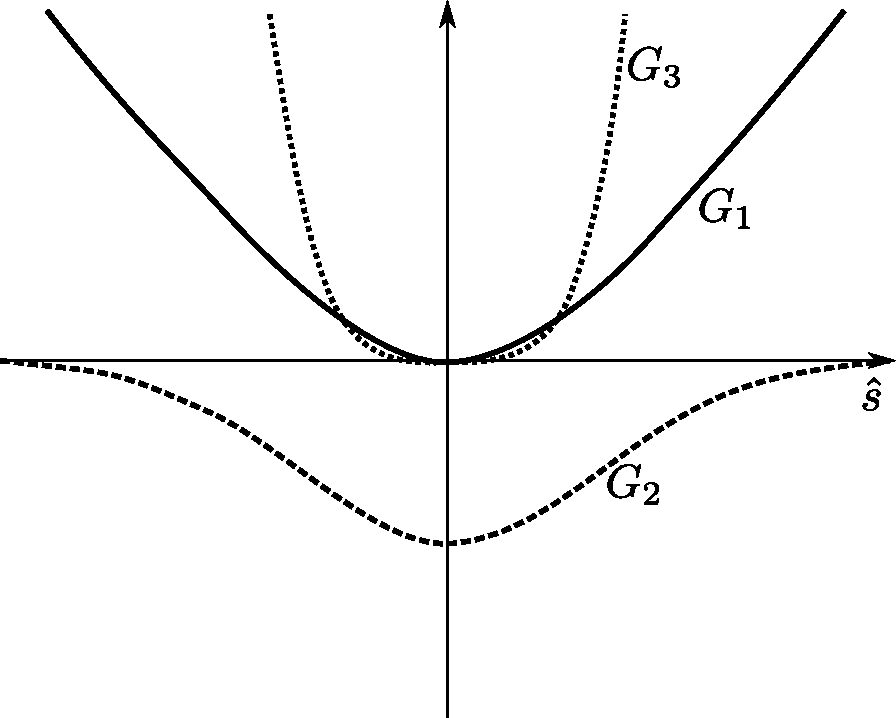
\includegraphics[width=4.5cm]{./img/contrast_functions.pdf}
    \vspace{-0.5cm}
 	\caption*{\hspace{5cm}\textit{\tiny{Source: Hyv\"arinen, 2001}}}
 \end{figure}
 
 \begin{equation*}
 	\smaller
 \begin{array}{lll}
 	G_1(\hat{s}) = \frac{1}{a} \log \cosh (a \cdot \hat{s}) 
 	\;\;& \;\;G_2(\hat{s}) = -\exp \Big( -\frac{(\hat{s})^2}{2} \Big)
 	& \;\;G_3(\hat{s}) = \frac{1}{4} (\hat{s})^4
	\end{array}
 \end{equation*}
 Any even, non-constant and non-quadratic (contrast) function $G$ can be used for ICA
 
 \question{When to choose which contrast function?}
 
 \end{frame}

\begin{frame}
\slidesonly{
\frametitle{Common contrast functions:}
}
\slidesonly{
	\smaller
	\begin{tabular}{ccc}
		$G_1(\hat{s}) = \frac{1}{a} \log \cosh (a \cdot \hat{s})$ & $G'_1(\hat{s}) = \tanh{(a\hat{s})}$ & $G''_1(\hat{s}) = a (1 - \tanh^2{(a\hat{s})})$\\[7pt]
		\multicolumn{3}{c}{general purpose} \\[25pt]
		$G_2(\hat{s}) = -\exp \Big( -\frac{(\hat{s})^2}{2} \Big)$ & $G'_2(\hat{s}) = \hat{s} \exp{(-\frac{(\hat{s})^2}{2})}$ & $G''_2(\hat{s}) = (1-(\hat{s})^2) \exp{(-\frac{(\hat{s})^2}{2})}$ \\[7pt]
		\multicolumn{3}{c}{good for ``super''-Gaussian sources with many ``outliers''} \\[25pt]
		$G_3(\hat{s}) = \frac{1}{4} (\hat{s})^4 $ & $G'_3(\hat{s}) = (\hat{s})^3$ & $G''_3(\hat{s}) = 3(\hat{s})^2$  \\[7pt]
		\multicolumn{3}{c}{kurtosis: good for ``sub''-Gaussian sources with few ``outliers''}
	\end{tabular}
}
\notesonly{
\begin{itemize}
    \item general purpose:
    \begin{itemize}
        \item $G_1(\hat{s}) = \frac{1}{a} \log \cosh (a \cdot \hat{s})$
        \item $G'_1(\hat{s}) = \tanh{(a\hat{s})}$
        \item $G''_1(\hat{s}) = a (1 - \tanh^2{(a\hat{s})})$
    \end{itemize}
    \item for ``super''-Gaussian sources with many ``outliers'':
    \begin{itemize}
        \item $G_2(\hat{s}) = -\exp \Big( -\frac{(\hat{s})^2}{2} \Big)$
        \item $G'_2(\hat{s}) = \hat{s} \exp{(-\frac{(\hat{s})^2}{2})}$
        \item $G''_2(\hat{s}) = (1-(\hat{s})^2) \exp{(-\frac{(\hat{s})^2}{2})}$
    \end{itemize}
    \item kurtosis: good for ``sub''-Gaussian sources with few ``outliers'':
    \begin{itemize}
        \item $G_3(\hat{s}) = \frac{1}{4} (\hat{s})^4 $
        \item $G'_3(\hat{s}) = (\hat{s})^3$
        \item $G''_3(\hat{s}) = 3(\hat{s})^2$
    \end{itemize}
\end{itemize}
}
\end{frame}

\begin{frame}
cf. lecture slides for optmization of negentropy using contrast functions.
\end{frame}

\begin{frame}
\question{How do we evaluate ICA?}\\

-cf. https://research.ics.aalto.fi/ica/icasso/
\end{frame}


\mode*

\clearpage

%\section{References}
%\begin{frame}[allowframebreaks] \frametitle{References}
	%\scriptsize
	%\bibliographystyle{plainnat}
	%\bibliography{bibliography}
%\end{frame}

\end{rightcolumn}
\end{paracol}

\end{document}
